\chapter[Introduction]{Introduction}
\setcitestyle{citesep={,\,\thechapter.}}
%   Introduction to the introduction: a short version (of only a few paragraphs) of the thesis' aims, research questions, contribution, objectives and findings.
%    State the overarching topic and aims of the thesis in more detail
%    Provide a brief review of the literature related to the topic (this will be very brief if you have a separate literature review chapter)
%    Define the terms and scope of the topic
%    Critically evaluate the current state of the literature on that topic and identify your gap
%    Outline why the research is important and the contribution that it makes
%    Outline your epistemological and ontological position
%    Clearly outline the research questions and problem(s) you seek to address
%    State the hypotheses (if you are using any)
%    Detail the most important concepts and variables 
%    Briefly describe your methodology
%    Discuss the main findings
%    Discuss the layout of the thesis

%    Does the first line of the introduction discuss the problem that your thesis is addressing and the contribution that it is making?
%    Does the introduction provide an overview of the thesis and end with a brief discussion on the content of each chapter?
%    Does the introduction make a case for the research?
%    Have the research questions/problems/hypotheses been clearly outlined (preferably early on)?
Electron paramagnetic resonance (EPR) is a spectroscopic technique to probe the interactions of unpaired electrons to the surrounding molecular environment. EPR has been employed to gain information on, for example, the structure and dynamics of proteins, organic-based radicals, transition metals, radical reactions, electron transfer processes, and metallo-enzymes. As a magnetic resonance technique, EPR requires an incident microwave magnetic field perpendicular to a static magnetic field.\cite{weil2007electron} Sensitivity is greatly enhanced by the use of microwave cavities, where the sample can be placed in a region of strong microwave magnetic field while minimizing electric field losses as illustrated in Fig.~\ref{fig:cavity}. These resonators have been developed to be general-purpose and are commercially available. However, many opportunities exist in instrumentation development for improvement to the quality of EPR data and to extend the applicability of EPR to samples that cannot currently be studied. 

\begin{figure}[ht]
 \centering
 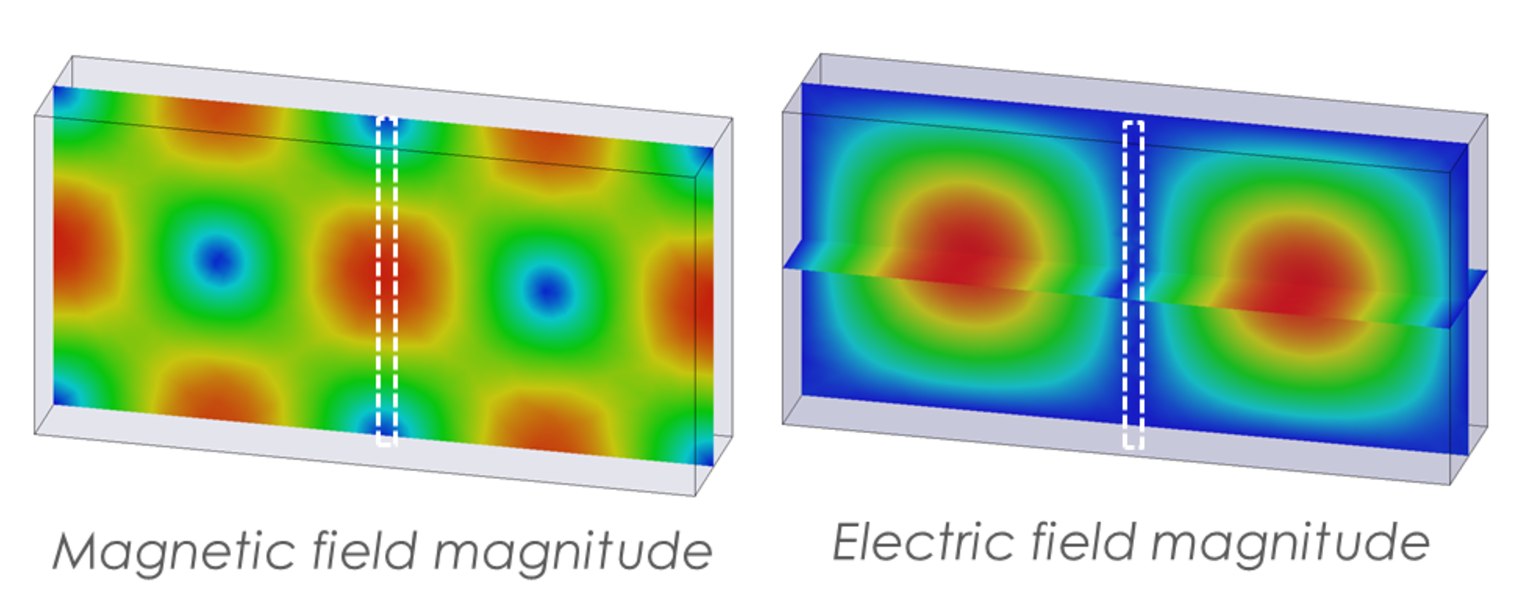
\includegraphics[width=0.85\textwidth]{Kapitel/Ch1-images/Cavity.eps}
 \caption[Standard TE$_{102}$ Caivty.]{The electric and magnetic field is shown for a standard TE$_{102}$ rectangular cavity. The placement of the sample is indicated by the white dashed area.}
 \label{fig:cavity}
\end{figure}

This work focuses on the development of application-specific microwave resonators to solve three challenges of modern EPR spectroscopy. Specifically, the three challenges investigated in this dissertation are tp: (i) Improve the microwave magnetic field homogeneity for pulse EPR at Q-band frequencies; (ii) Enhance the sensitivity of thin-film samples in the THz-bandgap by the implementation of meta-materials; (iii) Improve the absolute sensitivity at X-band frequencies for the study of protein single-crystals with volumes less than 30~nl.

\hspace{1em}
\noindent \paragraph*{Improving the microwave magnetic field homogeneity for pulse EPR at Q-band frequencies.}
With the inclusion of arbitrary waveform generators to modern EPR spectrometers, it has become increasingly important to have control over the excitation profile of the sample. \cite{DOLL201418,WILI201826} The excitation profile becomes crucial as the pulse sequences become more complex \cite{MILIKISYANTS200948,C7CP01488K,C6CP03067J,BREITGOFF2019106560} or when performing spin-spin distance measurements with radicals of different saturation profiles. \cite{C8CP01276H} Typically, a cosine dependence of the magnetic field along the sample axis exists, for example, in the conventional cylindrical TE$_{\text{102}}$ cavity shown in Fig.~\ref{fig:cavity}. As such, the sample experiences different excitation profiles which can limit the sensitivity and quality of pulse data. This is improved by the implementation of loop-gap resonators, but these geometries required smaller samples that limit concentration sensitivity. Herein, geometries that bridge the gap between cavities and loop-gap resonators are explored. By improving of the homogeneity of the microwave magnetic field\cite{HydeUFRev2019} and increasing the resonator bandwidth, an enhancement for frozen solution pulse EPR experiments is demonstrated. Such experiments are used to determine the principal values of the $g$-tensor or, using ELDOR-detected NMR (EDNMR), ESEEM, and/or HYSCORE spectroscopies, access hyperfine and quadrupole principal values of coupled nuclei. \cite{Harmer2009}

\hspace{1em}
\noindent\paragraph*{Enhancing the sensitivity of thin-film samples in the THz-bandgap by the implementation of meta-materials.}
Performing EPR at extreme microwave frequencies (up to 1~THz; THz-bandgap) requires high concentrations of samples since single-mode cavities are not geometrically feasible due to manufacturing and sample handling constraints. Usually, samples are formed into pellets and placed in the instrument for measurement. \cite{NEHRKORN201710} For many samples, such as powder or high concentrations of frozen proteins, this treatment is acceptable. However, for thin-films of paramagnetic materials, such as the study of metal-oxides for electronic and photonic devices, this is not feasible. \cite{oxidesurface} This investigation of meta-materials at THz-bandgap frequencies was driven by this need.

Herein, the meta-material consists of an array of split-ring resonators that cover the surface of a 12~mm diameter quartz glass. The meta-material removes the cross-sectional geometry constraints which are dictated by the wavelength of the frequency allowing for more sample, and therefore more EPR signal, at extremely high microwave frequencies. The use of meta-materials at THz frequencies has been previously studied from a context of strong- and weak-coupling between the spin resonance and frequency-dependent meta-material characteristics.\cite{SchneiderEPR,BOERO2013133,Scalari1323} However, these studies do not have an interest in the EPR signal and only seek to use the spin transitions to study light-matter interactions. In this work, we use the frequency-domain Fourier-transform EPR experiment to measure the interactions between the meta-material and EPR signal. A lumped-circuit transmission-line model describing the system was formulated to reproduce the complex interactions between the magnetic susceptibility of the sample and the frequency-dependent meta-material. Such interactions become increasingly important as the resonant probe geometry volume approaches the sample volume and in multi-wavelength probe designs found at higher frequencies. \cite{grinbergVHF}

\hspace{1em}
\noindent\paragraph{Improving the absolute sensitivity at X-band frequencies for the study of protein single-crystals with volumes less than 30~nl.}
Absolute sensitivity remains a challenge in EPR spectroscopy. This is especially true at X-band frequencies (9.5~GHz) where the majority of commercial EPR systems operate. By increasing the absolute sensitivity for sample volumes less than 30~nl a spectrocsopist could perform multi-frequency EPR using the same sample at X-band and high frequencies, such as W-band (94~GHz). 

This work focuses on the application of single-crystal EPR to protein crystals which are severely size limited by the availability of only small crystals. Crystal volumes are in the nanoliter to sub-nanoliter ranges, which are typical for X-ray crystallography diffraction studies but cannot be used in EPR due to lack of sensitivity. Typically, high-frequency EPR is utilized when the volume of a sample is limited. \cite{grinbergVHF} Although commercially available, high-frequency spectrometers are not readily available in most laboratories.

As a direct application, the resonant geometry developed here is employed to study [FeFe]-hydrogenase in the stable catalytic intermediate of H$_{ox}$ in protein single-crystals with dimensions less than 3~nl. By studying proteins in single-crystals, the angular dependencies of the magnetic parameters can be obtained. These angular dependencies help build a complete picture of the chemical structure and function of the active site of an enzyme.\cite{NiFe1996,NiFe2000,NiFe2003}

This dissertation is compiled in the following way. In Chapter 2, the basic understanding of EPR and general concepts for this work is introduced. Each main chapter is self-contained with an introduction, methods, results, and conclusion section. In chapter 3, a uniform field re-entrant TE$_{\text{01U}}$ is investigated and experimental measurements are provided. Chapter 4 is concerned with thin-film samples in the 100~GHz to 1~THz frequency range (3.34-33.36~cm$^{-1}$ energy range; THz-bandgap) and the implementation of meta-material surfaces. An analytical transmission-line model is proposed to describe the interaction of the meta-material surface and sample. Experimental measurements and analytical calculations are compared. Chapter 5 introduces the self-resonant micro-helix for protein single-crystal studies and Chapter 6 uses this novel resonator to study the metallo-enzyme [FeFe]-hydrogenase in the stable catalytic intermediate of H$_{ox}$ in protein single-crystals with a volume less than 3~nl.

{\renewcommand{\bibsection}{\clearpage\section*{\bibname}\markboth{\bibname}{\bibname}}
\renewcommand{\bibname}{CHAPTER 1. REFERENCES}
\bibliographystyle{elsarticle-num}
\bibliography{Kapitel/Ch1-References}
}